%%
%% 研究報告用スイッチ
%% [techrep]
%%
%% 欧文表記無しのスイッチ(etitle,jkeyword,eabstract,ekeywordは任意)
%% [noauthor]
%%

\documentclass[submit,techrep]{ipsj}
%\documentclass[submit,techrep,noauthor]{ipsj}



\usepackage[dvipdfmx]{graphicx}
\usepackage{latexsym}

\def\Underline{\setbox0\hbox\bgroup\let\\\endUnderline}
\def\endUnderline{\vphantom{y}\egroup\smash{\underline{\box0}}\\}
\def\|{\verb|}

\setcounter{巻数}{53}%vol53=2012
\setcounter{号数}{10}
\setcounter{page}{1}


\begin{document}


\title{データベース及び演習\\
(2023年7月31日)}

\etitle{Database and Exercises \\ (version 2012/10/12)}

\affiliate{IPSJ}{情報処理学会\\
IPSJ, Chiyoda, Tokyo 101--0062, Japan}


\paffiliate{JU}{情報処理大学\\
Johoshori Uniersity}

\author{水谷祐生}{Yusei Mizutani}{IPSJ}[joho.taro@ipsj.or.jp]

\begin{abstract}
本稿は,情報処理学会論文誌ジャーナルに投稿する原稿を執筆する際,および論
文採択後に最終原稿を準備する際の注意点等をまとめたものである.大きく分け
ると,論文投稿の流れと,\LaTeX と専用のスタイルファイルを用いた場合の論
文フォーマットに関する指針,および論文の内容に関してするべきこと,するべ
きでないことをまとめたべからずチェックリストからなる.本稿自体も \LaTeX 
と専用のスタイルファイルを用いて執筆されているため,論文執筆の際に参考に
なれば幸いである.
\end{abstract}

%
%\begin{jkeyword}
%情報処理学会論文誌ジャーナル,\LaTeX,スタイルファイル,べからず集
%\end{jkeyword}
%
%\begin{eabstract}
%This document is a guide to prepare a draft for submitting to IPSJ
%Journal, and the final camera-ready manuscript of a paper to appear in
%IPSJ Journal, using {\LaTeX} and special style files.  Since this
%document itself is produced with the style files, it will help you to
%refer its source file which is distributed with the style files.
%\end{eabstract}
%
%\begin{ekeyword}
%IPSJ Journal, \LaTeX, style files, ``Dos and Dont's'' list
%\end{ekeyword}

\maketitle

%1
\section{機能概要}
このアプリケーションには
\begin{itemize}
  \item 「作成者名」「部屋名」「部屋の説明」を入力した後、「作成」ボタンを押すことで部屋を作成する機能
  \item 部屋の説明欄を編集する機能
  \item  タグを作成する機能
  \item 作成したタグを部屋の参加者に割り当てる機能
  \item 参加者を追加する機能
  \item 参加者を削除する機能
  \item 参加者カードの「編集」を押すことで「名前」または「コメント」を編集する機能
  \item 部屋の参加者の受付をするかしないかを決める機能
  \end{itemize}
  といった機能が実装されている.

\section{利用技術}
\subsection{Next.js}
\subsubsection{Next.jsとは}
Next.jsとはReactをベースに開発された、フロントエンドフレームワークである.

Next.jsでは画像・レンダリングを最適化する。最適化するメリットとしてページの読み込み速度が高速になることである.また、読み込み速度の高速化はSEOにも効果がある.このようにNext.jsを利用することで、Webページ閲覧時のユーザー体験を向上させる、作成したページを誰かに見てもらいやすくなるといったメリットがある.

\subsubsection{Reactとは}
ReactとはFacebook社が開発したWebサイト上のUIパーツを構築するためのJavaScriptライブラリである.また、JSX記法と呼ばれる構文が採用されていて、これにより一つのファイル内でHTMLタグに対する動きを操作することができる.
同様のJavaScriptのライブラリとしてVue.js、Angularなどが挙げらるが、Reactは中でも世界的に圧倒的な導入率を誇ってている。
\subsection{ChakraUI}
Chakra UIとは、UIコンポーネントライブラリの1つで、自前でCSSを書かなくてもパラメータ指定でスタイルを記述でき、デザインに一貫性を持たせることができる。
再利用可能なコンポーネントも多く用意されていて、アラートダイアログやドロワーメニュー、トーストなど自前で作ろうとすると大変なものも簡単に実現できる。また、レスポンシブ対応も容易に行うことができるため誰でも簡単に洗練されたデザインのUIを構築することが可能である.

\subsection{TypeScript}
TypeScriptとはオープンソースかつ、JavaScriptを拡張して開発されたプログラミング言語であり、Microsoftによって開発された.

基本的な文法はJavaScriptと大した変化はないが、大きな違いとして型付けができるかどうかが挙げられる.

従来までのJavaScriptには型付けがない、つまり動的型付けといって実行時にプログラム側が勝手に数値型、文字型を判定するため実行時のエラーの存在に気づかず思わぬバグに繋がることがあった.この問題を解決するためTypeScriptでは静的型付けといって実行前にプログラマーがあらかじめ型を設定できるようにした.また静的型付けによって、変数の説明ができるため大規模な開発においてソースコードの可読性という観点からも恩恵を受けることができる.


\subsection{Go}
\subsubsection{Go言語とは}
Go言語とは、シンプルかつ高速な処理が可能なプログラミング言語であり、Google社によって開発された.
コードをシンプルかつにそして高速に動作させるというコンセプトの元に開発されたため、他の言語には実装されている機能、例えば「継承」や「ジェネリクス」などが実装されていない.そのため、誰が書いても似たようなコードになり、アプリケーションの管理を簡単にすることができる.
\subsubsection{Ginとは}
GinとはGo言語の中でも人気のあるWebフレームワークである.

Ginには高速なパフォーマンス、JSONのリクエストのバリデーション、ルーティングのグループ化、エラー管理、組み込みのレンダリング、といった特徴があるため、Ginなしで開発するよりもより高速、簡単にWebアプリケーションやAPIサーバーを開発することができる.

\subsubsection{API}
APIとは「Application Programming Interface」の略である.言葉通りに意味を解釈すると、アプリケーションをプログラミングするためのインターフェースという意味である.簡単に説明すると、APIとはソフトウェアにAPIという外部とやりとりする窓口であり、外部アプリとコミュニケーションや連携ができるものである.

\section{システム設計}

\subsection{システム概要}
今回のアプリのシステム構成図は図1のようになっており、UI描写専用のNext.jsのサーバーとMySQLサーバーとやり取りを行うGoサーバー今回はフレームワークとしてGinを使用しているためGinサーバーの二つが連携することによって動作するようになっている.具体的な連携方法として、HTTPメソッドでやり取りをを行っており、今回はNext.jsサーバーがGET、POST、PUT、DELETEメソッドにパラメーターやボディーに変数を乗せてGinサーバーにリクエストを送り、バックエンド側でそれに応じたデータベースに対する操作を行い、最終的な結果をNext.jsサーバー、つまりフロントエンドにレスポンスとして返している.

\begin{figure}[htbp]
  \centering
 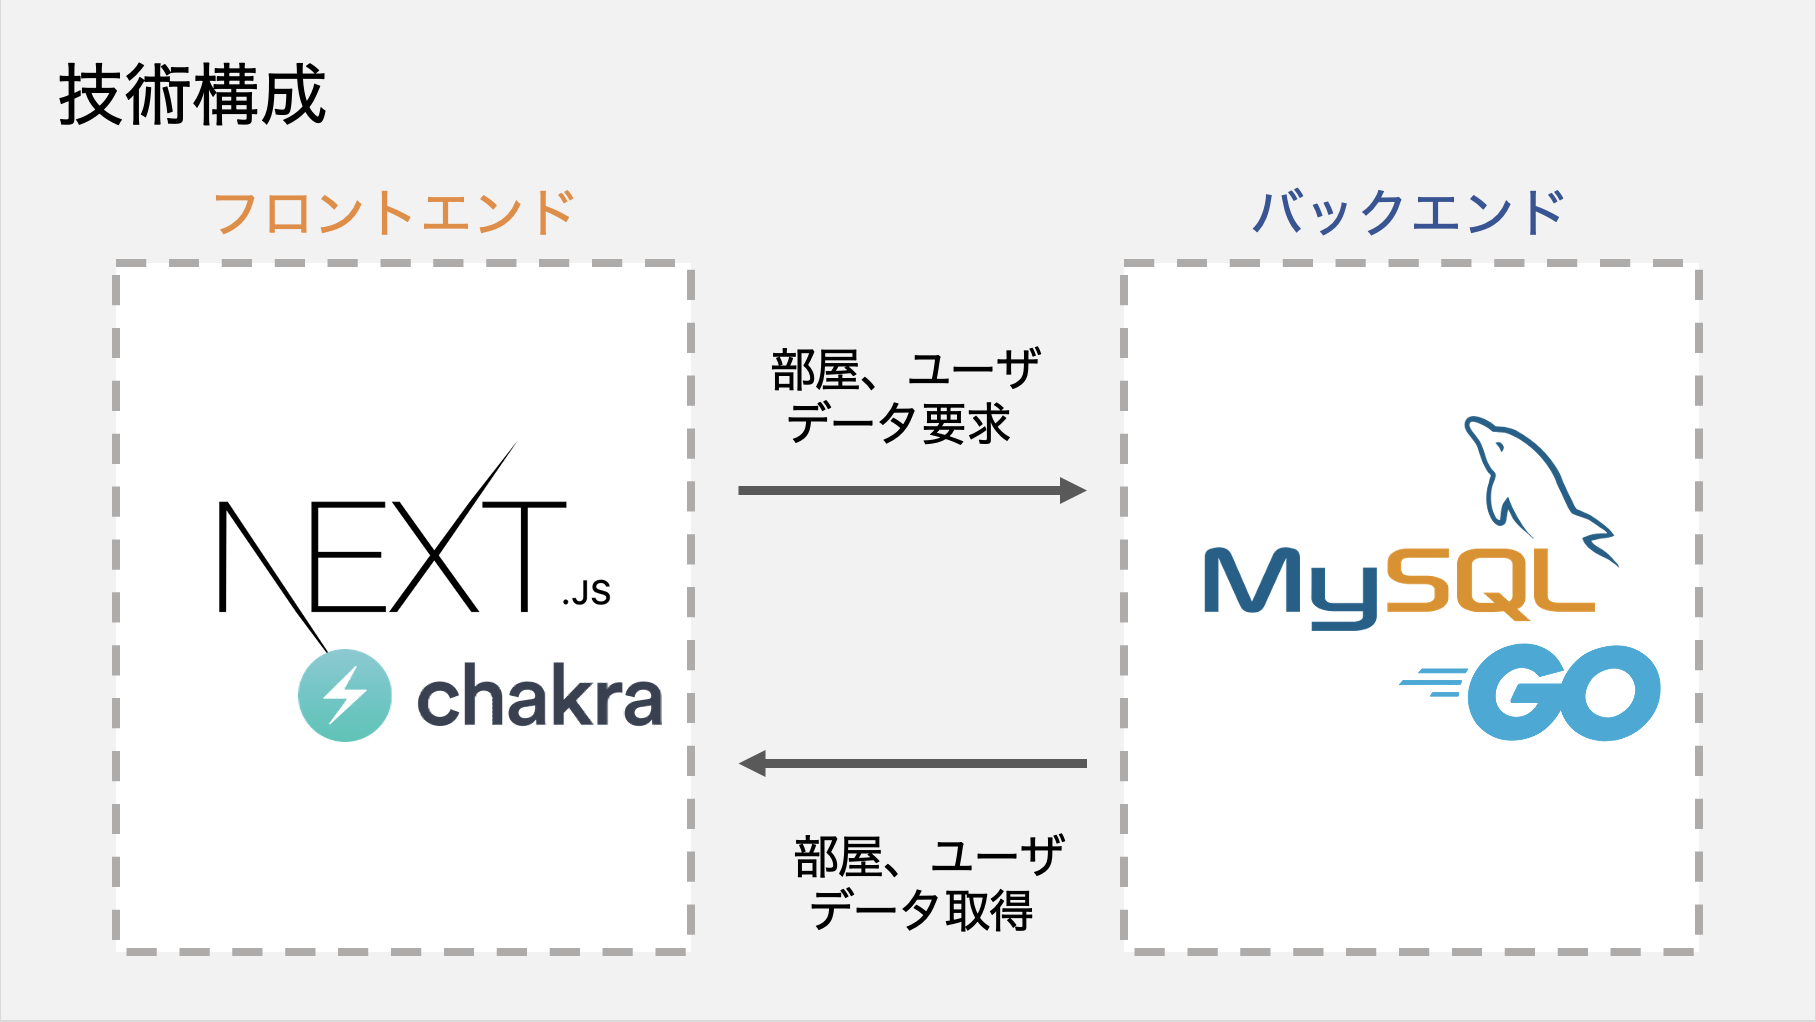
\includegraphics[width=8cm]{./images/technical_configuration.jpg}
  \caption{システム構成図}
  \label{fig:sample}
\end{figure}

\subsection{技術選定の意図}
\subsubsection{Next.js}
Next.jsはデフォルトでサーバーを持っているため、create react appを利用して開発した際に設定しなくてはならないWebpackやbabelの記述の負担を減らすことができるため採用した.

\subsubsection{ChakraUI}
ChakraUIはCSSを記述しなくとも洗練されたデザインのUIコンポーネントを扱うことができるため、フロントエンド側でのデータ処理やクリック時の処理に時間を咲くことができる.すなわち、システム的な機能実装に集中することができるため採用した.

\subsubsection{Go}
他にもPython、Javaなどが候補に上がったが、中でもGo言語はGormといったORMマッパーや、Ginといった強力なWebフレームワークが備わっているため、APIサーバーを作成するために便利なパッケージが備わっている.それゆえに、Go言語を採用した

\subsubsection{MySQL}
今回のアプリの性質上、RDBを用いると最も容易にデータ管理を行うことができると考えたため採用した.



\subsection{画面遷移}

\begin{figure}[htbp]
  \centering
 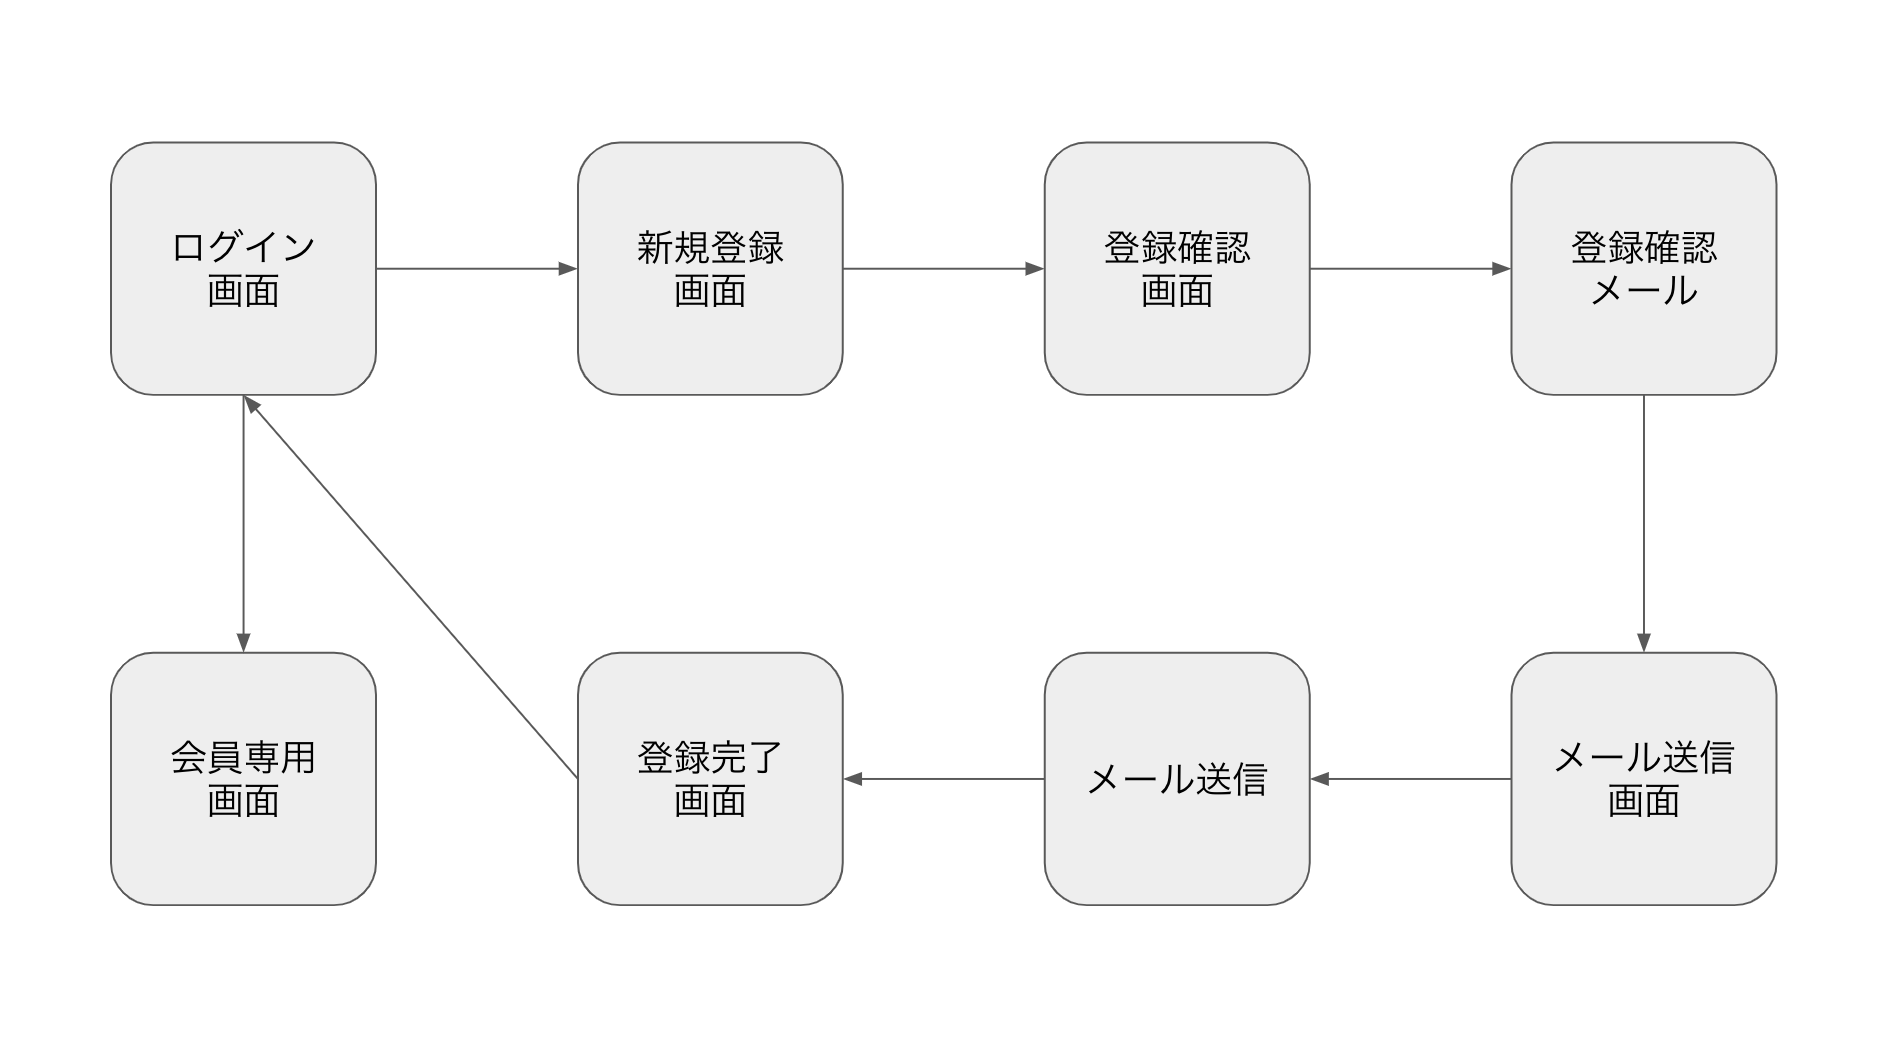
\includegraphics[width=8cm]{./images/screen_transition.jpg}
  \caption{画面遷移の図}
  \label{fig:sample}
\end{figure}

図2は今回のプログラムにおける画面遷移を表したものであり、以下にその詳細を記す.
\subsubsection{部屋作成の動き}
\begin{enumerate}
  \item 「部屋一覧画面」で「新しく部屋を作る」ボタンをおして「部屋追加画面」に遷移する
  \item 「部屋追加画面」で作成者名、部屋名、部屋の説明を入力して「作成」ボタンをおす
  \item  ボタンを押したと同時に部屋を新規作成、部屋画面に遷移する
 \end{enumerate}
といった流れになっている.

\subsubsection{部屋参加の動き}
\begin{enumerate}
  \item 部屋に入っている人から「部屋画面」に表示されているQRコードまたはURLを共有してもらう
  \item 「部屋画面」の「参加者を追加する」ボタンを押すと、ドロワーが表示される
  \item  ドロワーにある名前、コメントを入力してから「参加する」ボタンを押す

 \end{enumerate}
といった流れになっている.


図3は今回のサンプルプログラムにおける管理者が行える操作を表したものであり、以下にその詳細を記す.

\begin{enumerate}
  \item 管理者専用の画面の新規登録ボタンを押すと図2の新規登録画面に遷移する
  \item 管理者専用画面の中のの会員一覧の更新ボタンを押すと、登録された会員情報の内容を修正することができる更新画面へ遷移する
  \item  管理者専用の画面の中の会員一覧に存在する削除ボタンを押すことで、登録された会員情報を削除することができる、削除確認画面に遷移する
  \end{enumerate}
といった流れになっている.

\subsection{データベース設計}
今回作成したサービスでは三つのテーブルが存在する.
一つ目は、日本の都道府県を閲覧する際に使用されるkenテーブル、二つ目は、名前、メールアドレス、パスワードなど会員情報を管理するためのmemberテーブル、三つ目はメールを用いて本登録を行っていないユーザーを仮登録として保持しておくためのprememberテーブル、これら三つのデータをMariaDB/MySQLを通して行うことでシステムを動かしている.

以下に、それぞれのテーブルについて記述していく.

\subsubsection{kenテーブル}
\begin{verbatim}
CREATE TABLE ken (
    id      SMALLINT,
    ken     VARCHAR(10),
    PRIMARY KEY (id)
);
\end{verbatim}
上のSQL文は都道府県のデータを格納するために定義されたテーブルである.

フィールドについて説明すると、idとはカラムを識別するため主キー、kenは都道府県の名前をを格納している.

\subsubsection{memberテーブル}
\begin{verbatim}
CREATE TABLE member (
    id          
    MEDIUMINT UNSIGNED NOT NULL AUTO_INCREMENT,
    username   	VARCHAR(50),
    password   	VARCHAR(128),
    last_name  	VARCHAR(50),
    first_name 	VARCHAR(50),
    birthday   	CHAR(8),
    ken         SMALLINT,
    reg_date   	DATETIME,
    cancel      DATETIME,
    PRIMARY KEY (id)
);
\end{verbatim}
上のSQL文は本登録されたユーザーのデータを格納するために定義されたテーブルである.

以下、それぞれのフィールドについて説明する

\begin{enumerate}
  \item idとはカラムを識別するため主キー、またUNSIGNED NOT NULLAUTO\_INCREMENTとは、カラムを追加される時に自動で順番にidフィールドに数字を格納するという意味である.ただし、0は受け付けない.
  \item usernameフィールドは文字列で定義されていて、カッコ内にある50とは、50バイト分の文字列まで格納できるという意味である.
 \item usernameフィールドは文字列で定義されていて、カッコ内にある50とは、50バイト分の文字列まで格納できるという意味である.
  \item passwordフィールドは文字列で定義されていて、カッコ内にある128とは、128バイト分の文字列まで格納できるという意味である.
   \item last\_nameフィールドは文字列で定義されていて、カッコ内にある50とは、50バイト分の文字列まで格納できるという意味である.
    \item first\_nameフィールドは文字列で定義されていて、カッコ内にある50とは、50バイト分の文字列まで格納できるという意味である.また、出身地の情報は都道府県を直接入れているわけではなく、kenテーブルで定義されているidを参照して管理している.こうすることでデータ量の多い都道府県の文字列よりもデータ量の少ない数値で管理できるためサーバーの負荷を軽減することができる.

  \item kenフィールドは数値で定義されていて、SMALLINTとは、-32,767 から 32,767 までの小さい整数を格納することができる意味である.
 \item reg\_dateフィールドはDARETIME型で定義されていて、YYYY-MM-DD形式で格納されている
 \item cancelフィールドはDARETIME型で定義されていて、YYYY-MM-DD形式で格納されている  \end{enumerate}

\subsubsection{prememberテーブル}
\begin{verbatim}
CREATE TABLE premember (
    id          
    MEDIUMINT UNSIGNED NOT NULL AUTO_INCREMENT,
    username   	VARCHAR(50),
    password   	VARCHAR(128),
    last_name  	VARCHAR(50),
    first_name 	VARCHAR(50),
    birthday   	CHAR(8),
    ken         SMALLINT,
    link_pass  	VARCHAR(128),
    reg_date   	DATETIME,
    PRIMARY KEY (id)
);
\end{verbatim}
上のSQL文は仮登録されたユーザーのデータを格納するために定義されたテーブルである.

基本的なフィールドはmemberテーブルとあまり差異はないが、一部異なる部分もある.link\_passフィールドである.このフィールドは本登録テーブルと仮登録テーブルの情報を結びつけるためのフィールドである.

%2.3
\subsection{システム詳細}



\begin{table}[h]
 \caption{各処理における分岐の表}
 \label{table:SpeedOfLight}
 \centering
  \begin{tabular}{lllll}
   \hline
   type & action & ボタン & 処理 & 表示画面 \\
   \hline \hline
   無し &&& 認証 & 会員画面TOP \\
   無し &&& 未認証 & ログイン画面 \\
   authenticate & - & - & 認証処理OK & 会員画面TOP \\
   authenticate & - & - & 認証処理NG & ログイン画面 \\
   regist & form & - & - & 入力画面 \\
   regist & confirm & - & 入力チェックOK & 確認画面 \\
   regist & confirm & - & 入力チェックNG & 入力画面 \\
   regist & complete & 戻る & - & 入力画面 \\
   regist & complete & 登録 & INSERT & 完了画面 \\
   modify & form & - & - & 入力画面 \\
   modify & confirm & - & 入力チェックOK & 確認画面 \\
   modify & confirm & - & 入力チェックNG & 入力画面 \\
   modify & complete & 戻る & - & 入力画面 \\
   modify & complete & 登録 & UPDATE & 完了画面 \\
   delete & confirm & - & - & 入力画面 \\
   delete & complete & - & DELETE & 完了画面 \\
   modify & - & - & ログアウト処理 & ログイン画面 \\
   \hline
  \end{tabular}
\end{table}

表2は,typeとactionの値によって,振り分けられるときの条件を表したものである.次の画面へ遷移されるときリンクをクリックして画面を表示させるときか、送信ボタンを押して画面を表示させるときのいずれかである. 送信ボタンを押して、画面遷移する場合は、HTTPのGETメソッドにより、パラメーターをURLに載せて、サーバに送信している.送信ボタンを押して画面遷移する場合は、HTTP の POST メソッドを用いて、ユーザーからは確認できないよう安全に値が送信される.

ここで、GETメソッドとPOSTメソッドの違いについて説明する.

GETメソッドはURLにパラメータを含めることで、サーバーに情報を送るHTTPリクエストの一つである.主に、あるページを取得するためにサーバーにリクエストを送る際にこのメソッドが用いられる.

POSTメソッドとはパラメータをリクエストヘッダーに含めることで、サーバーとデータのやり取りを行うHTTPリクエストの一つである.GETメソッドと明確に異なる点として、サーバーに送った情報がユーザーには見ることができない点が挙げられる.この特徴によりPOSTメソッドは、主にデータを追加する際、今回のサンプルプログラムだとユーザーの仮登録、本登録をする際、個人情報などといった第三者に見られてはいけない情報を送信する際に用いられる.

メソッドの決め方としては、\$this-\>type の値でメソッドが決まり、メソッドの内部では\$this-\>action の値で処理を振り分けていく.また,送信ボタンが二つある画面では,ボタンの名称を振り分けに利用している.

\subsection{変数設計}

\subsection{各画面設計}
各画面はQuickForm2、Smarty により、PHPファイルをもとに自動生成されている.

画面描写に必要なファイルはsmatryディレクトリのtemplatesディレクトリ内にある.tplファイルである.これらのファイルを読み込むことで、画面を描写することができる.

\subsubsection{ログイン画面}
ログイン画面の描写には、login.tplを用いている

index.phpの情報を参照することでセッション管理を行なっていて、ログイン済みであると認証されなかった場合は、このページに遷移するようになっている.

また、入力欄に入力した内容をブラウザ側で保持しつつ出るために、\$form.username.labelには,ユーザー名を格納し、\$form.username.htmlはユーザー名の入力欄、HTMLのコードに置き換わる.同様に、\$form.password.labelはパスワード名に、\$form.password.htmlはパスワー ド入力欄にHTMLのコードに置き換わる.

\subsubsection{仮登録表示画面}
画面の描写にはpremember.tplが用いられる.

新規登録画面から確認画面でユーザーが登録情報を確認した後に遷移する画面であり、メールを送信した旨を伝えるための画面である.

\subsubsection{会員専用画面}
画面の描写にはmember\_top.tplが用いられる.

ログインを終えた会員とindex.phpにセッションが残っている場合は子も画面に遷移する.

\subsubsection{管理者専用画面}
画面の描写にはsystem\_login.tplが用いられる.

管理者用のパスワードを入力し、認証を終えると、このページに遷移する.
会員一覧へのリンクは\$SCRIPT\_ NAME?type=list\& action=formとなり\$ SCRIPT\_ NAMEはsystem.phpに置き換わる。 クリックするとsystem.phpに対してtype=listとaction=formが送信され、会員一覧を表示する。

\section{実装}

\subsection{実装環境}
\begin{table}[h]
 \caption{用いたツール名とそのバージョンの表}
 \label{table:SpeedOfLight}
 \centering
  \begin{tabular}{ll}
   \hline
   名前 & バージョン  \\
   \hline \hline
  OS & macOS Venture バージョン 13.4 \\
  XAMPP &  7.4.28 \\
  PHP & 7.4.28 \\

   \hline
  \end{tabular}
\end{table}

今回は以上の表のような環境で動作確認を行なった.

\subsection{環境設定}
今回のサンプルプログラムを動作させるために必要なXAMPPの環境構築は以下のように行なった.

\begin{enumerate}
  \item 公式サイトからXAMPPをインストールする
  \item 設定を行い、XAMPPコントロールパネルを起動させる
  \item  WebサーバーであるApacheを起動させる
  \end{enumerate}
といった流れになっている.

次に実際に今回のシステムを動作させるためのプログラムの配置は以下の手順で行なった

\begin{enumerate}
  \item 「環境構築から実践的なシステム作成まで完全習得! PHP7+MariaDB/MySQL マスターブック」に記されているサンプルデータにアクセスする
  \item そこにあるSection77の内容を引用するために、XAMPPディレ クトリにphp\_libsを作成し、htdocsとphp\_libsに引用したサンプルプログラムをすべて移す.
データの Section77 に入っているすべてのファイルを移す。
  \item  コピペしたフォルダにあるファイルにアクセス権を付与する
  \end{enumerate}
  
  
  MySQLの初期設定は以下の手順で行なった.
\begin{enumerate}
  \item sqlフォルダを作成する
  \item サンプルプログラムのSection76、Section86からにあるSQLファイルをコピーして、sqlフォルダに格納する
  \item MySQLにアクセスし、予め、データベースやテーブル、初期ユーザーをインサートしておく
  \end{enumerate}
といった流れになっている.

今回のサンプルプログラムでは、メールを受け取って、本登録を完了する機能が実装されている.そこで、gmailのメール受け取りに関する設定が必要になっため、その手順を以下に記す.


\begin{enumerate}
  \item gmailのWebページにアクセスする
  \item 右上の歯車のアイコンをクリックする
  \item 押すと、「全ての設定を表示」という項目が表示されるためそれをクリックする
  \item 「メール転送とPOP/IMAP」をクリックする
  \item 「IMAPアクセス」のステータスを「IMAP を有効にする」に変更する
  \end{enumerate}
  
   \begin{figure}[htbp]
  \centering
 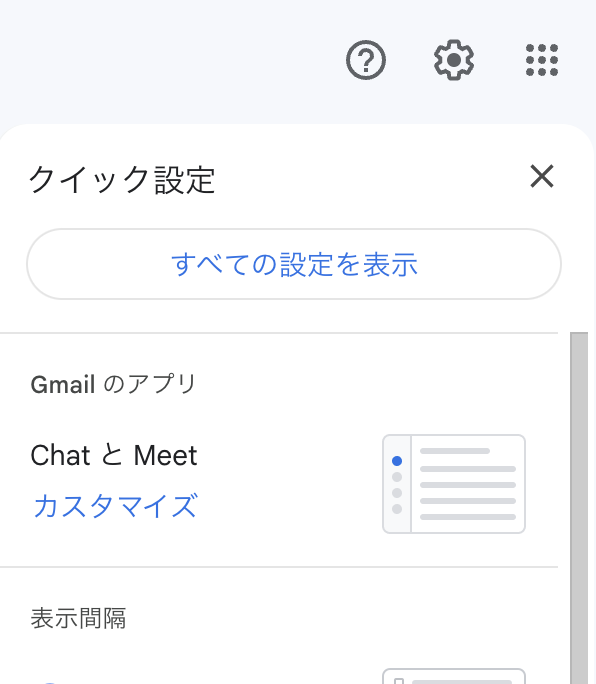
\includegraphics[width=8cm]{./images/all_setting.jpg}
  \caption{全ての設定を表示ボタンが表示されている画面の図}
  \label{fig:sample}
\end{figure}
  
  \begin{figure}[htbp]
  \centering
 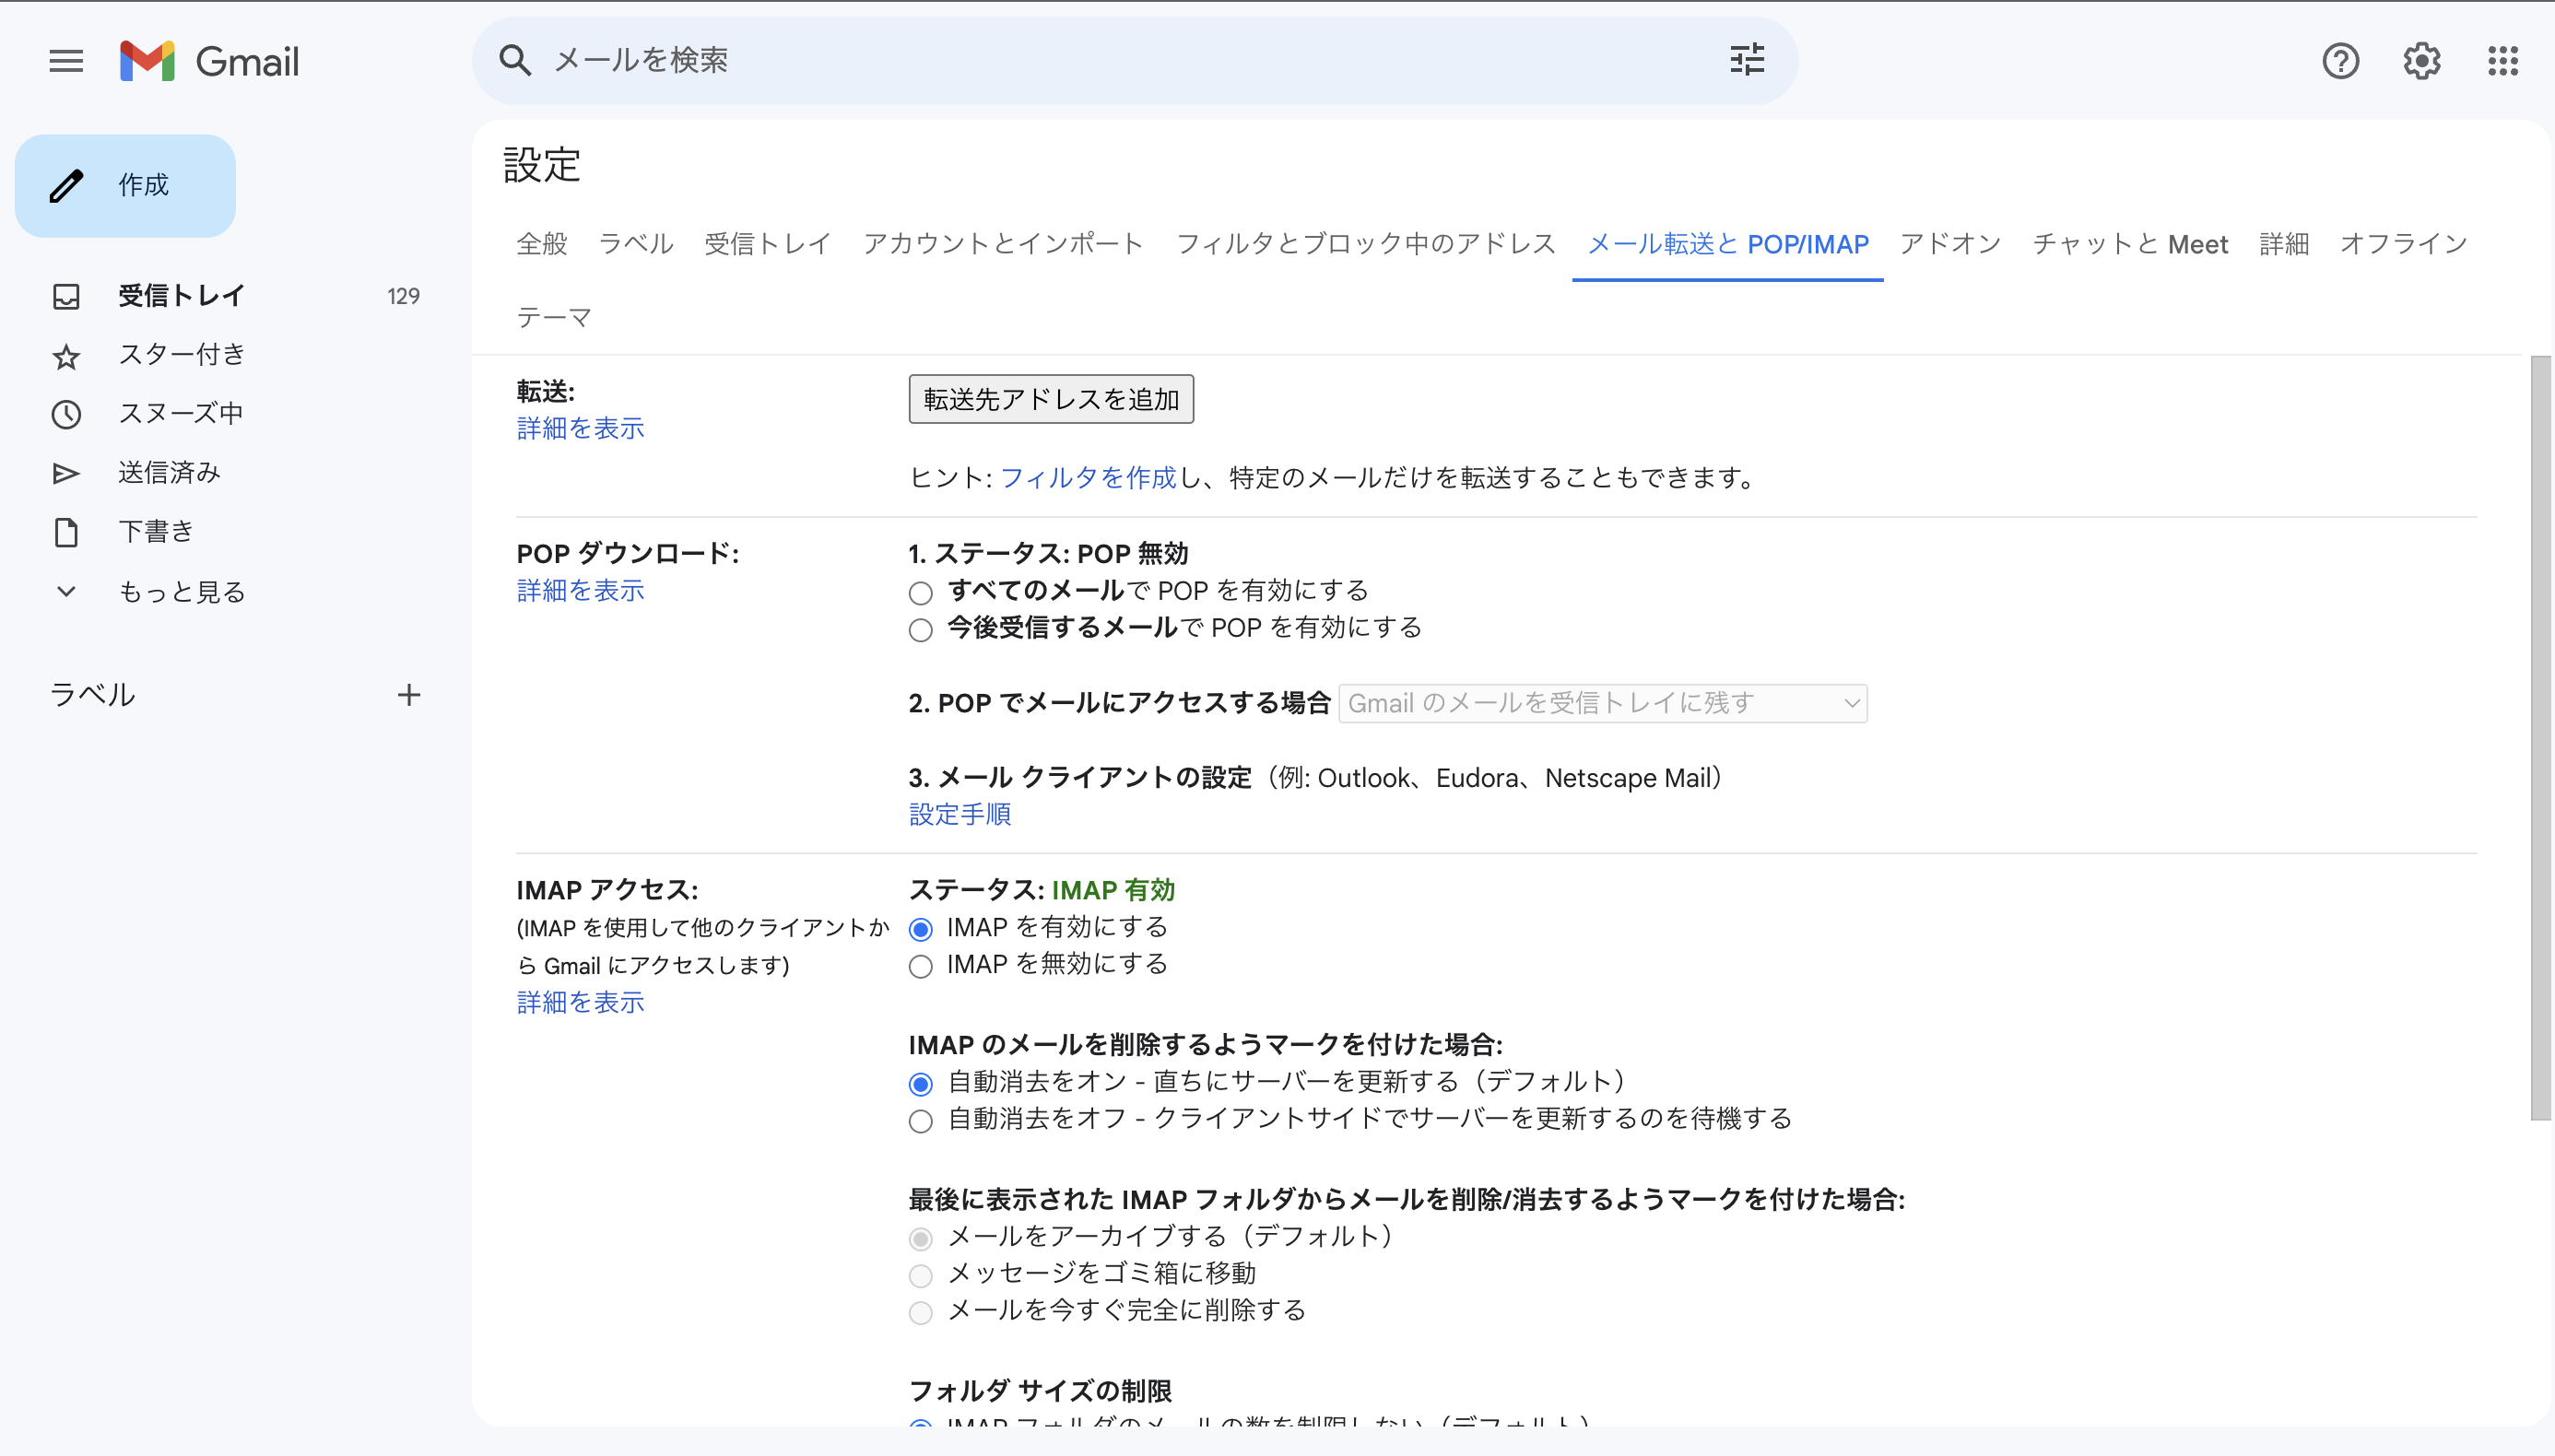
\includegraphics[width=8cm]{./images/pop_imap.jpg}
  \caption{IMAPを有効にした時の画面図}
  \label{fig:sample}
\end{figure}

以上の手順を踏むと、Gmailのコンソール画面のうちIMAPアクセス」のステータスを「IMAP を有効にする」に変更でき、IMAPサーバーからPOPサーバーにメールの内容を送信できるようになる.

また、本来Smatryを利用する際はインストールするまでに必要な手順を踏む必要があるが、サンプルプログラムを引用することでその必要は無くなったため、説明は省略することにする.

\subsection{動作検証}
画面遷移の説明の際に用いた図2の手順を踏んで行なった.
まずは一般会員に関する動作検証を行なった.
\begin{enumerate}
  \item ログイン画面では自分の入力した内容がフォームにもそのまま反映されるかを検証した
  \item 新規登録画面ではログイン画面同様、フォームにもそのまま反映されるかに加えデータベースに格納されている都道府県情報が選択できているかを検証した
  \item 登録確認画面ではユーザーが新規登録画面で入力した値がprememberテーブルに格納され、表示できているか検証
  \item メール確認後、本登録が完了した旨を伝える画面が表示されるかを検証
  \item 再びログイン画面に遷移した時、新規登録で登録したメールアドレス、パスワードでログインを行えるか検証
   \item 会員専用画面で、登録内容の修正、削除、ログアウトが行えるか検証
  \item 「IMAPアクセス」のステータスを「IMAP を有効にする」に変更する
   \item 「メール転送とPOP/IMAP」をクリックする
  \item 「IMAPアクセス」のステータスを「IMAP を有効にする」に変更する
  \end{enumerate}
  
 次には管理者に関する動作検証を行なった.
\begin{enumerate}
  \item ログイン画面で管理者用のパスワードを入力することで管理者用のページに遷移することができるかを検証した
  \item 管理者ページから会員一覧ページに遷移できるか検証
  \item 会員一覧ページでは、会員情報を全て閲覧できるようになっているか、またそれを削除、修正することができるかを検証
  \item メール確認後、本登録が完了した旨を伝える画面が表示されるかを検証
  \item 再びログイン画面に遷移した時、新規登録で登録したメールアドレス、パスワードでログインを行えるか検証
  \end{enumerate}
  
  以上のように一般会員、管理者の動作検証を行ったところ、画面遷移や表示内容、処理について全く不具合が確認できなかったため、システムは正常に動作していると判断した.
  
\section{まとめ}
今回のサンプルプログラムではPHPとMySQLを連携させて作る簡単な会員登録アプリを作成した.普段、個人またはチームでアプリ開発に取り組む際は、便利なライブラリに頼ったり、Firebaseに認証機能を任せていたりしているためメール認証で使われるSMTPサーバー、POPサーバーについて深く知ることができたことはとても良い経験になった.

アプリ全体を通して、いつデータベースにアクセスして削除、追加、閲覧を行ったらよいのか、また、セッションとクッキーの管理、バリテーション、メール送信機能が実装されているため、基本的なアプリの流れを知ることができるアプリであった.

また、今回のアプリは新規登録を行なってログインをして、ログイン者専用ページを表示するといったとてもシンプルなものであったが、今後、会員専用ページに機能を拡張していくことでより面白いアプリにすることができる基盤となるアプリであるとも考えた.



%% 以下は無視されます

\begin{biography}
\profile{m}{情報 太郎}{1970年生.1992年情報処理大学理学部情報科学科卒.
1994年同大大学院修士課程了.同年情報処理学会入社.オンライン出版の研究
に従事.電子情報通信学会,IEEE,ACM 各会員}
%
\profile{n}{処理 花子}{1960年生.1982年情報処理大学理学部情報科学科卒.
1984年同大大学院修士課程了.1987年同博士課程了.理学博士.1987年情報処
理大学助手.1992年架空大学助教授.1997年同大教授.オンライン出版の研究
に従事.2010年情報処理記念賞受賞.電子情報通信学会,IEEE,IEEE-CS,ACM
各会員}
%
\profile{s}{学会 次郎}{1950年生.1974年架空大学大学院修士課程了.
1987年同博士課程了.工学博士.1977年架空大学助手.1992年情報処理大学助
教授.1987年同大教授.2000年から情報処理学会顧問.オンライン出版の研究
に従事.2010年情報処理記念賞受賞.情報処理学会理事.電子情報通信学会,
IEEE,IEEE-CS,ACM 各会員}
%
\end{biography}



\end{document}
